\subsection{Data Set}
Portrait data set is used in this paper. The portrait data set is used for image stylization, which is to segment the portrait in the selfie for style conversion. It is a simple single-target portrait segmentation problem that is suitable for experiments with the level set method to try to apply it the segmentation of complex scenes.
\begin{figure}[h]
    \centering
    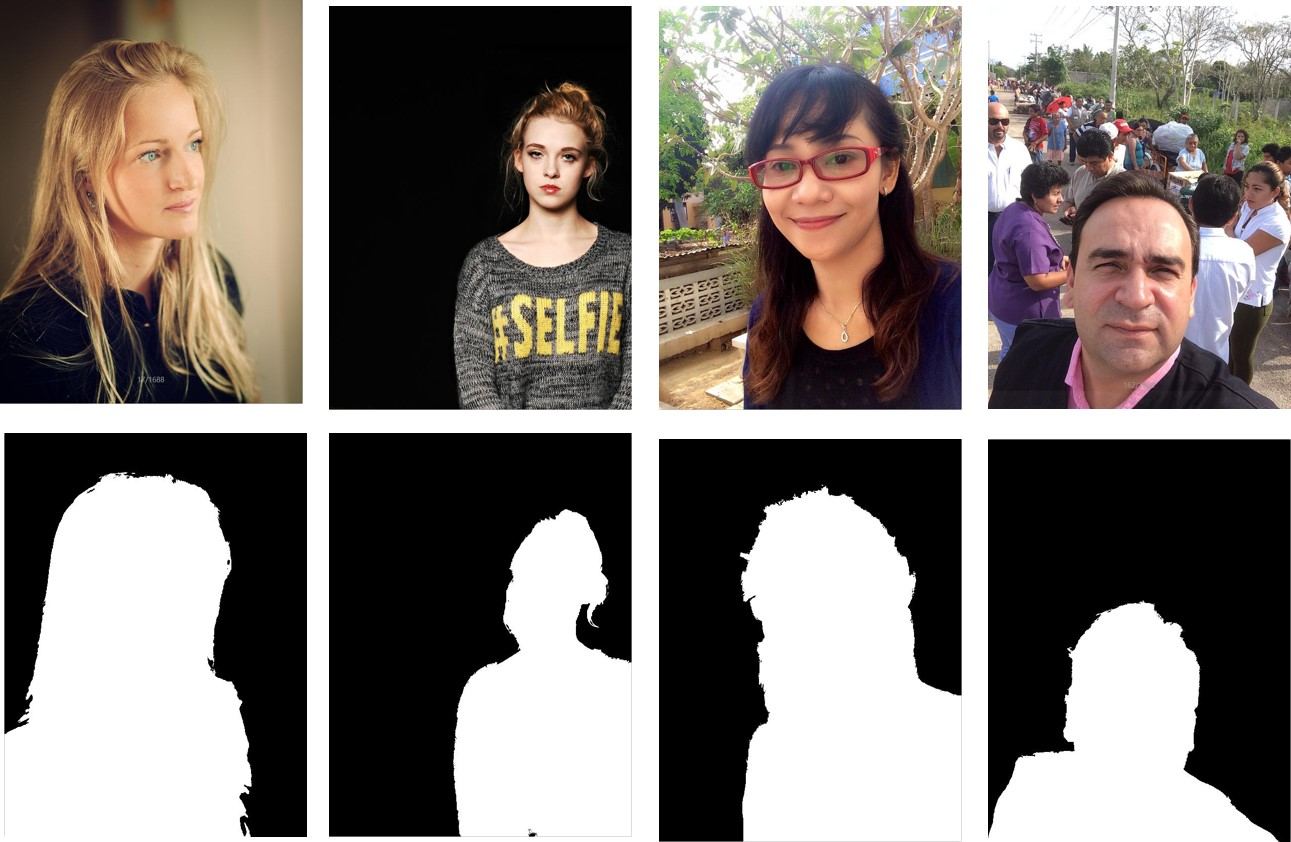
\includegraphics[width = 7cm]{figs/PortraitDataSet.jpg}
    \caption{Some images and ground truth of Portrait data set.}\label{fig: Some images and ground truth of Portrait data set}
\end{figure}
Some images and ground truth of portrait data set are shown in Fig. \ref{fig: Some images and ground truth of Portrait data set}. There are $1800$ portrait images in total, each of which is automatically scaled and cropped to $600\times800$, so every image is a standard portrait. The $1800$ labeled images data set was split into a $1500$ image training data set and a $300$ image testing data set by Shen et al. \cite{FCN:segmentation:shen2016automatic}, and this division is also used in this paper. Because the images in Portrait data set is labeled with Photoshop quick selection, there is some noise in ground truth, as shown in Fig. \ref{fig: Some noise in the Portrait data set}.
\begin{figure}[h]
    \centering
    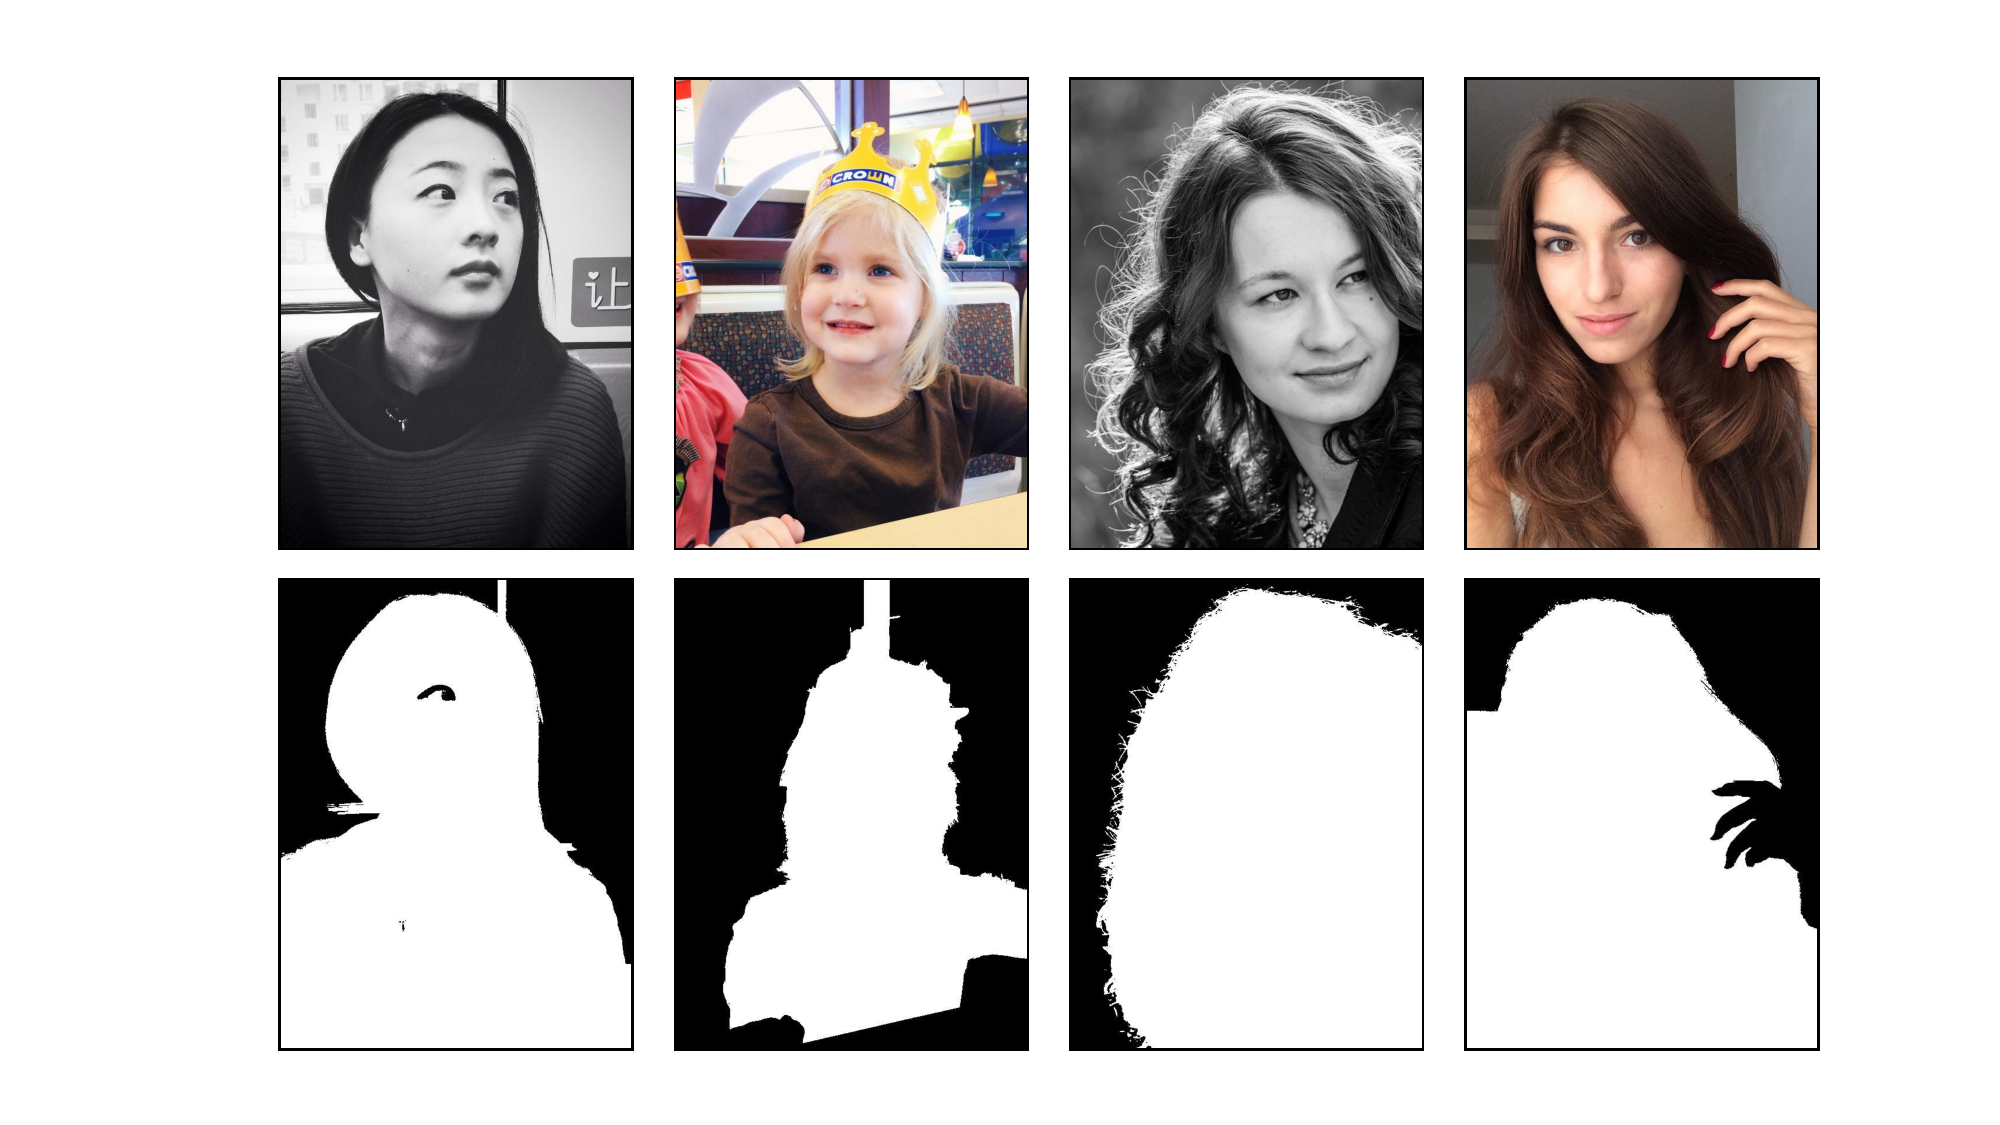
\includegraphics[width = 7cm]{figs/DataSetNoisy.eps}
    \caption{Some noise in the Portrait data set.}\label{fig: Some noise in the Portrait data set}
\end{figure}

\subsection{Evaluation Measure}
There is only one kind of segmentation target in this image segmentation task, only the regions of target need to be marked. So we only need to calculate the difference between the output regions of models and the regions of ground truth. The standard metric Interaction-over-Union (IoU) is selected to represent the segmentation error.
\begin{equation*}
    \text{IoU} = \frac{\text{Area}(\text{Output} \cap \text{Ground Truth})}{\text{Area}(\text{Output} \cup \text{Ground Truth})}
\end{equation*}
It is calculated by dividing the intersection area and the union area of the region of model output and ground truth . Finally, the mean IoU of $300$ testing images is used to verify the performance of models.
\subsection{Implementation}
All FCNs are trained with Caffe \cite{FCN:caffe:jia2014caffe}, and with all parameters given by Shen et al. \cite{FCN:segmentation:shen2016automatic}. The probability map is obtained from PortraitFCN and PortraitFCNplus which are trained with Portrait data set.
It can be seen from Fig. \ref{fig: Some results of the GAT} that it is already very close to the shape of the probability map at the second iteration, so the number of GAT iterations is set to $2$. The Level Set function $\phi$ is initialized with the probability map, and extended to intervals $[-200, 200]$. The same parameters are used in all testing images, and the parameters are listed int Table \ref{table: Parameters of the proposed method}.
\begin{table}[h]
    \centering
    \caption{Parameters of the proposed method.}\label{table: Parameters of the proposed method}
    \begin{tabular}{c|c|c}
        \hline
        \hline
        Parameter & Value & Reference \\
        \hline
        $\epsilon$ & 0.5 & Eq. \ref{eq: equation epsilon} \\
        $\sigma$ & 4 & Eq. \ref{eq: gaussian sigma} \\
        $\lambda_1$ & 20 & Eq. \ref{eq: Level Set 1-item} \\
        $\lambda_2$ & 20 & Eq. \ref{eq: Level Set 1-item} \\
        $\pi_1$ & 2*500 & Eq. \ref{eq: Level Set 2-item} \\
        $\pi_2$ & 2*500 & Eq. \ref{eq: Level Set 2-item} \\
        $\nu$ & 0.5*255*255 & Eq. \ref{eq: Level Set 3-item} \\
        $\mu$ & 1.0 & Eq. \ref{eq: Level Set 4-item} \\
        $\Delta t$ & 0.2 & Eq. \ref{eq: iter Level Set} \\
        \hline
        \hline
    \end{tabular}
\end{table}
\footnote{The codes are available at https://github.com/zsh965866221/LevelSet-ShapePrior-DeepLearning}

\subsection{Result and Analysis}\label{subsec: Result and Analysis}
In this paper, we mainly compare with Shen's method, which is equivalent to an attempt at image segmentation task with the combination of Level Set method and FCNs. FCN8s is a CNN structure proposed by J Long et al. \cite{FCN-original:long2015fully}, and trained with the Pascal VOC data set \cite{FCN:DataSet:Everingham15}. There are $21$ different classes in the Pascal VOC data set, but the Portrait data set used in this paper has noly $1$ class, so only the person class in FCN8s is used. The PortraitFCN is the retrain of FCN8s at Portrait data set. The PortraitFCNplus expands the $3$-channel of the original image into $6$-channel based on the PortraitFCN, adding the Mean Mask and Normalized x and y. The Mean Mask is shown is Fig. \ref{fig: The standard shape mask}. In this paper, we select the output of PortraitFCN and PortraitFCNplus as the probability maps respectively to verify the performance of the proposed Level Set method.
Finally, the performance comparison of different models at Portrait data set is show in Table \ref{table: Performance comparson of different models}, and the contour evolution process of proposed Level Set method at Portrait data set is shown in Fig. \ref{fig: The contour evolution process of proposed Level Set method at Portrait data set}.
\begin{table}[h]
    \centering
    \caption{Performance comparison of different models at Portrait data set.}\label{table: Performance comparson of different models}
    \begin{tabular}{c|c}
        \hline
        \hline
        \textbf{Methods} & \textbf{Mean IoU} \\
        \hline
        FCN(Person Class) & 73.09\% \\
        PortraitFCN & 94.20\% \\
        PortraitFCN + Proposed & 95.17\% \\
        PortraitFCNplus & 95.91\% \\
        PortraitFCNplus + Proposed & 95.74\% \\
        \hline
        \hline
    \end{tabular}
\end{table}
\begin{figure}[h]
    \centering
    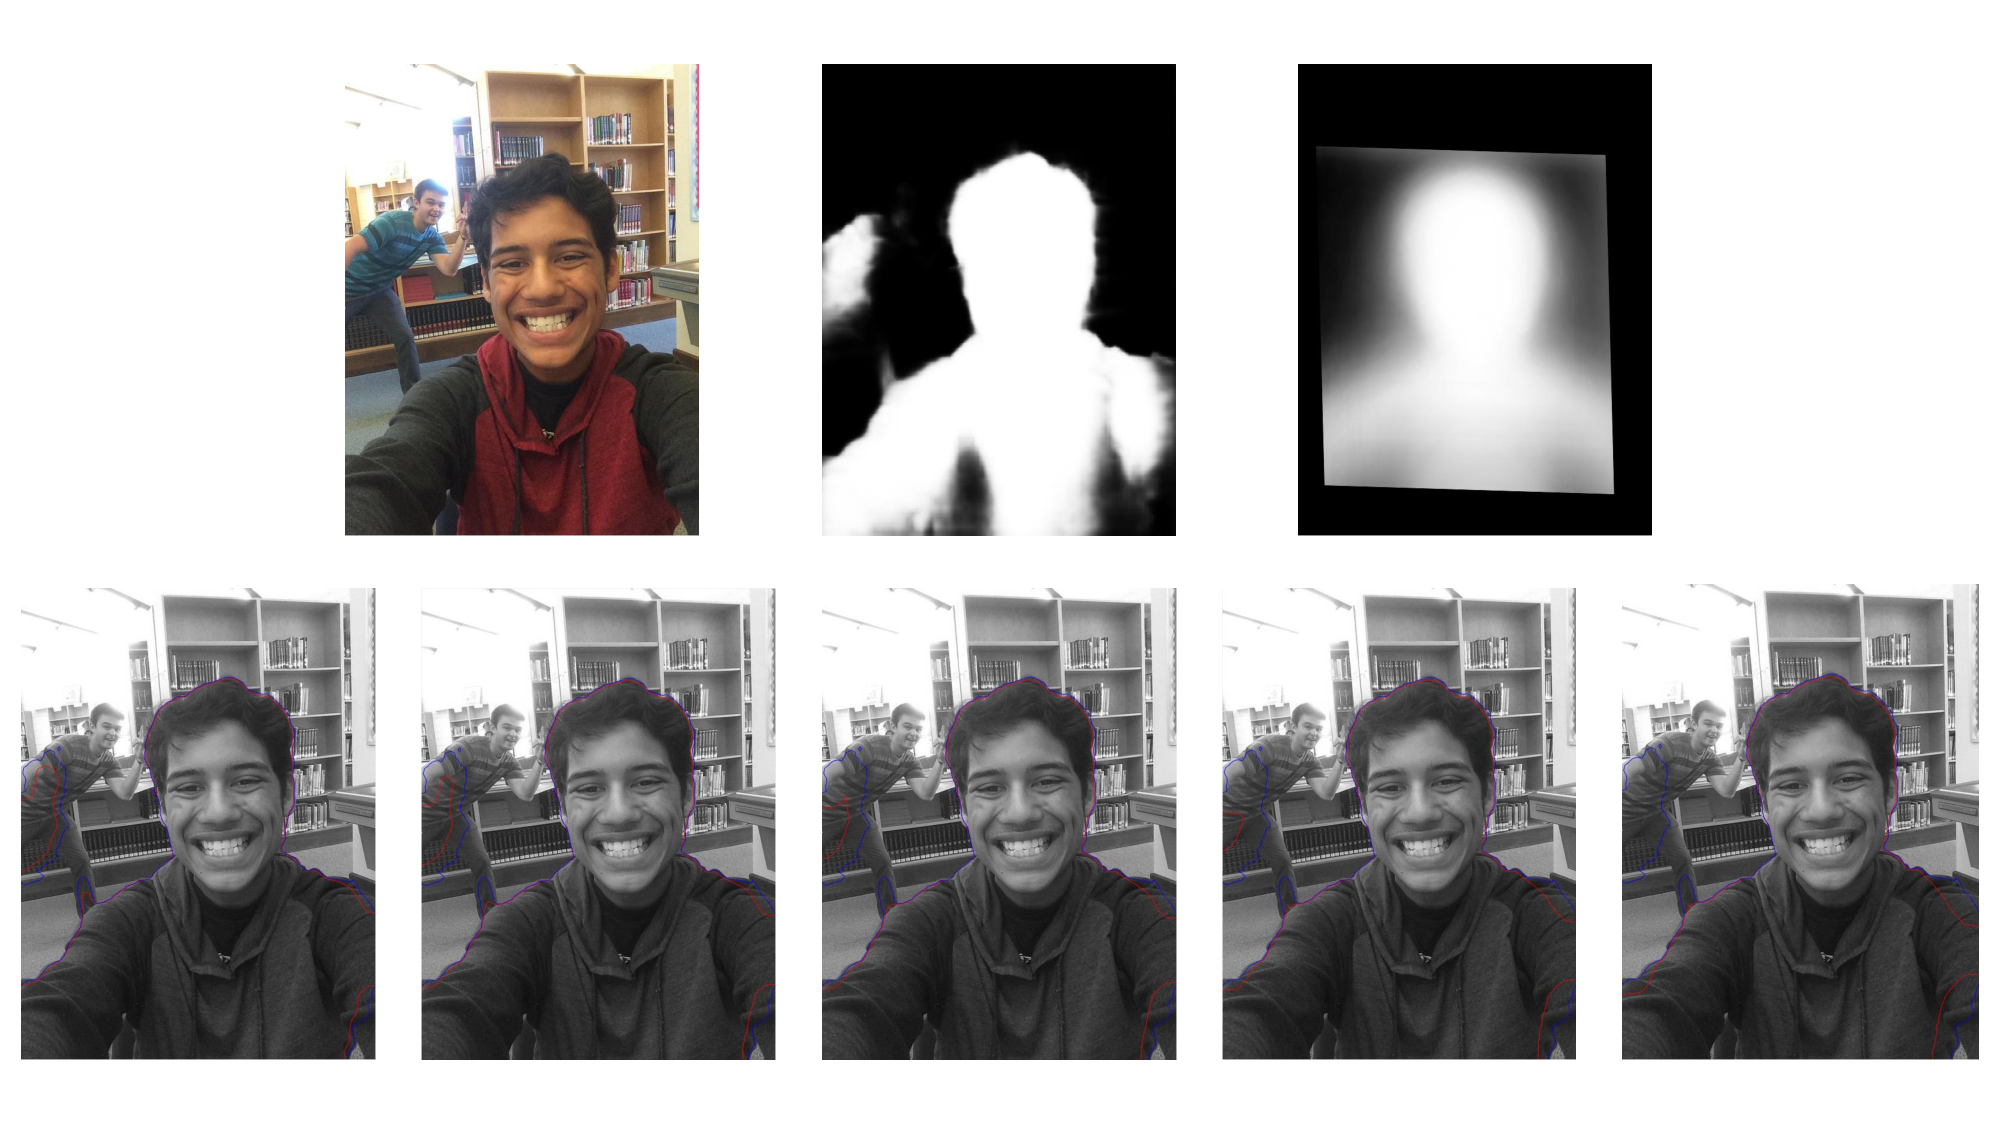
\includegraphics[width=9cm]{figs/LevelSet_Result.eps}
    \caption{The contour evolution process of proposed Level Set method at Portrait data set. The picture below is the evolution process. the blue curve is the contour by the probability map, and the red is the proposed Level Set method.}
    \label{fig: The contour evolution process of proposed Level Set method at Portrait data set}
\end{figure}

We can see from Table \ref{table: Performance comparson of different models} that, the proposed method has some improvement with PortraitFCN, but some weakening with PortraitFCNplus. As shown in Fig. \ref{fig: Some results of the GAT}, the output of PortraitFCN have some shortcomings list in Item. \ref{itemize: FCN shortcomings}, such as noisy, non-smooth, imprecise at boundary and no shape prior. The proposed method mainly to solve the problem of shape prior, so it is effective with PortraitFCN. However, with PortraitFCNplus, the mean mask has been added in the training process, and it has achieved a great performance at most of the pictures. Because of the imprecise of the corrected shape prior, the original probability map information would be disturbed during the evolution of the Level Set, that degrades the performance. We can see from Fig. \ref{fig: The contour evolution process of proposed Level Set method at Portrait data set}, the regions far from the corrected prior shape would be erased during the iterative process. But the region in the lower right corner of the image is considered to have a low probability, so it is also erased.

\subsection{The Results of Different Reference Information}
In this subsection, a series of experiments is conducted to verify the effect of different reference information on the segmentation result. We select an image form Portrait data set to explain, and the image, the probability map from PortraitFCN and the corrected shape prior are shown in Fig. \ref{fig: The image, the probability map and the corrected shape prior for experiments}.
\begin{figure}[h]
    \centering
    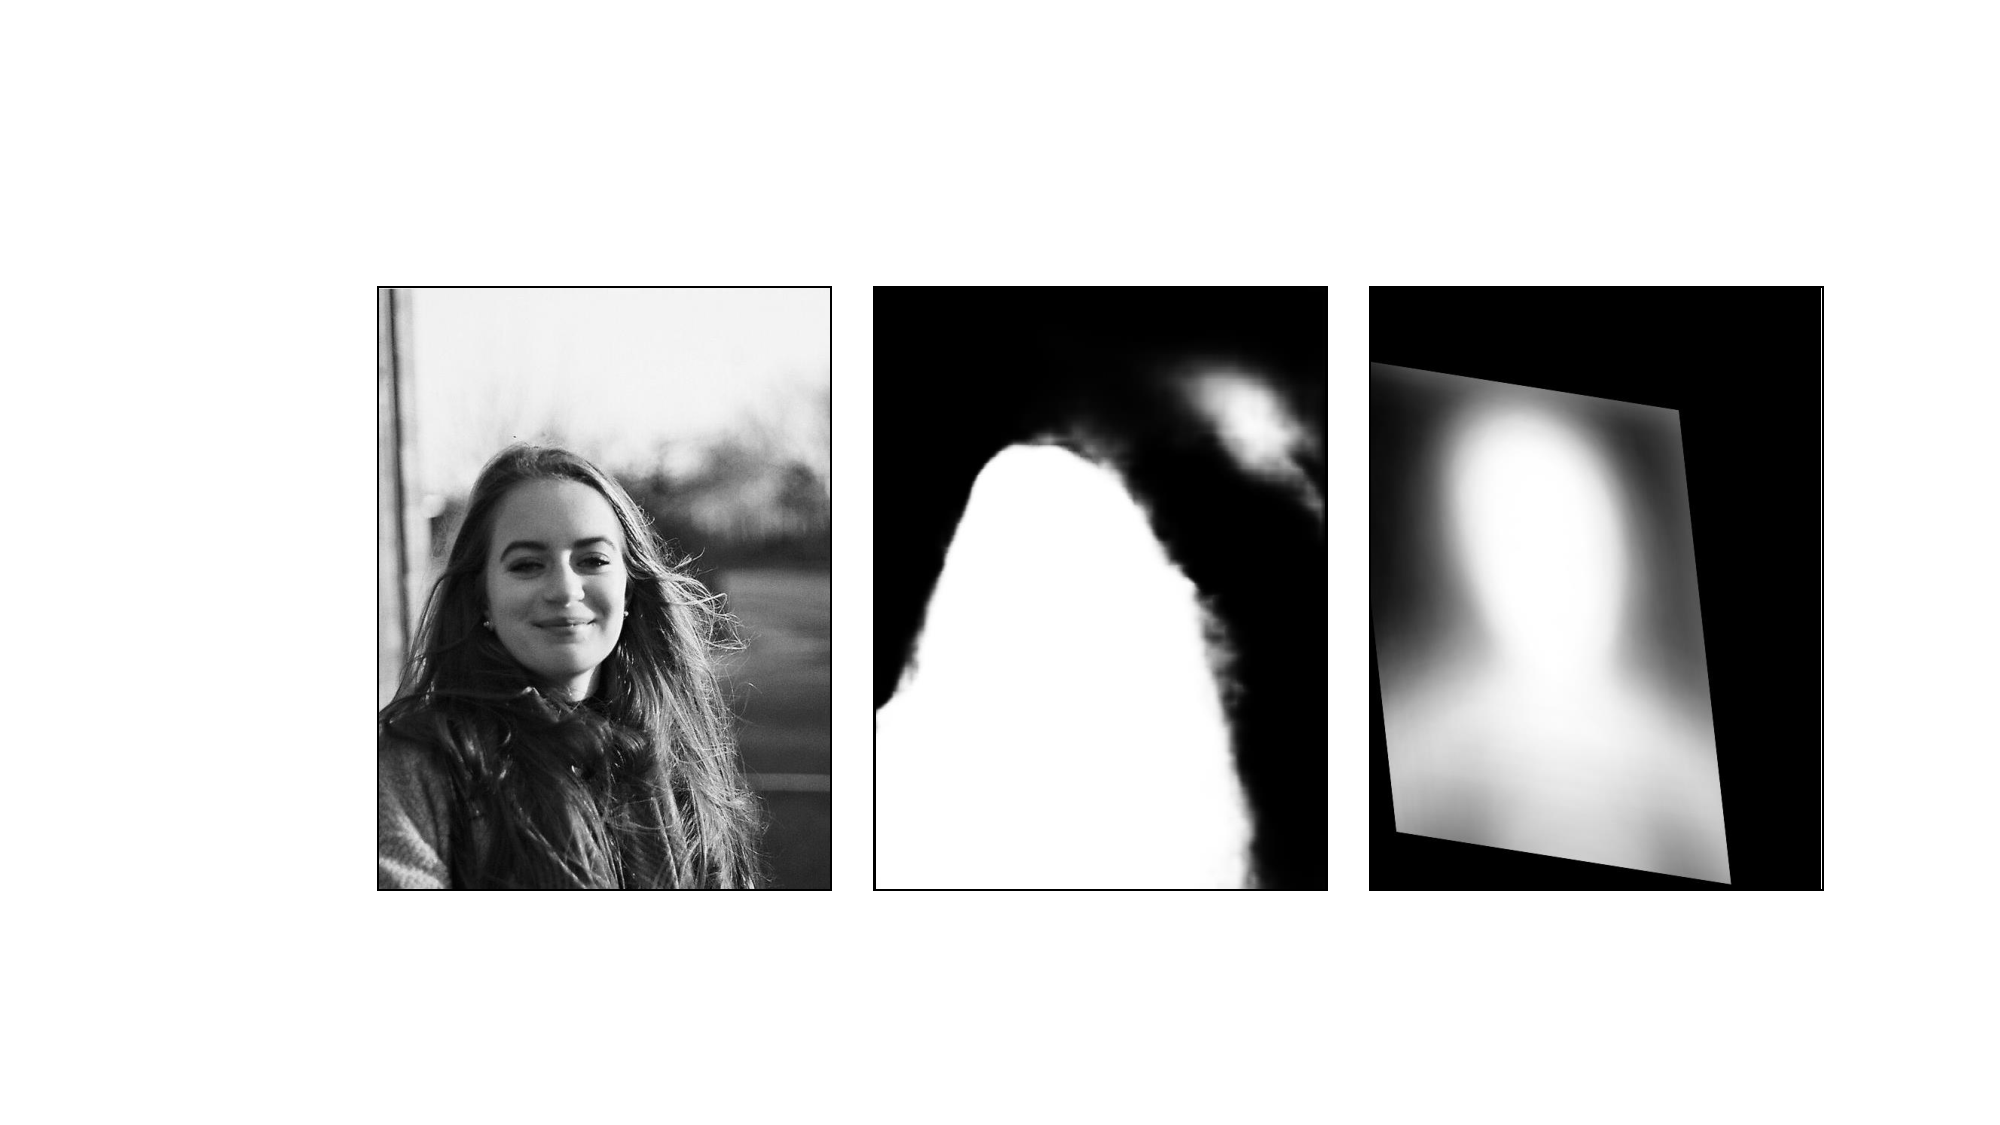
\includegraphics[width=7cm]{figs/DifferentInformation_image.eps}
    \caption{The image, the probability map and the corrected shape prior for experiments.}
    \label{fig: The image, the probability map and the corrected shape prior for experiments}
\end{figure}

\subsubsection{Experiment $1$}
The reference information selected in Experiment $1$ is just like the Subsection \ref{subsec: Level Set Method for Image Segmentation} above. It uses the original image and the probability map information in $\mathcal{E}_{\text{img}}$, so that the regions that are close to each other in pixels and satisfy the probability map are grouped together. And $\mathcal{E}_{\text{shape}}$ just uses the corrected prior shape, it ensures the similarity of the final segmentation and the corrected shape prior. The contour evolution process of Experiment $1$ is shown in Fig. \ref{fig: The contour evolution process of Experiment 1}.
\begin{figure}[h]
    \centering
    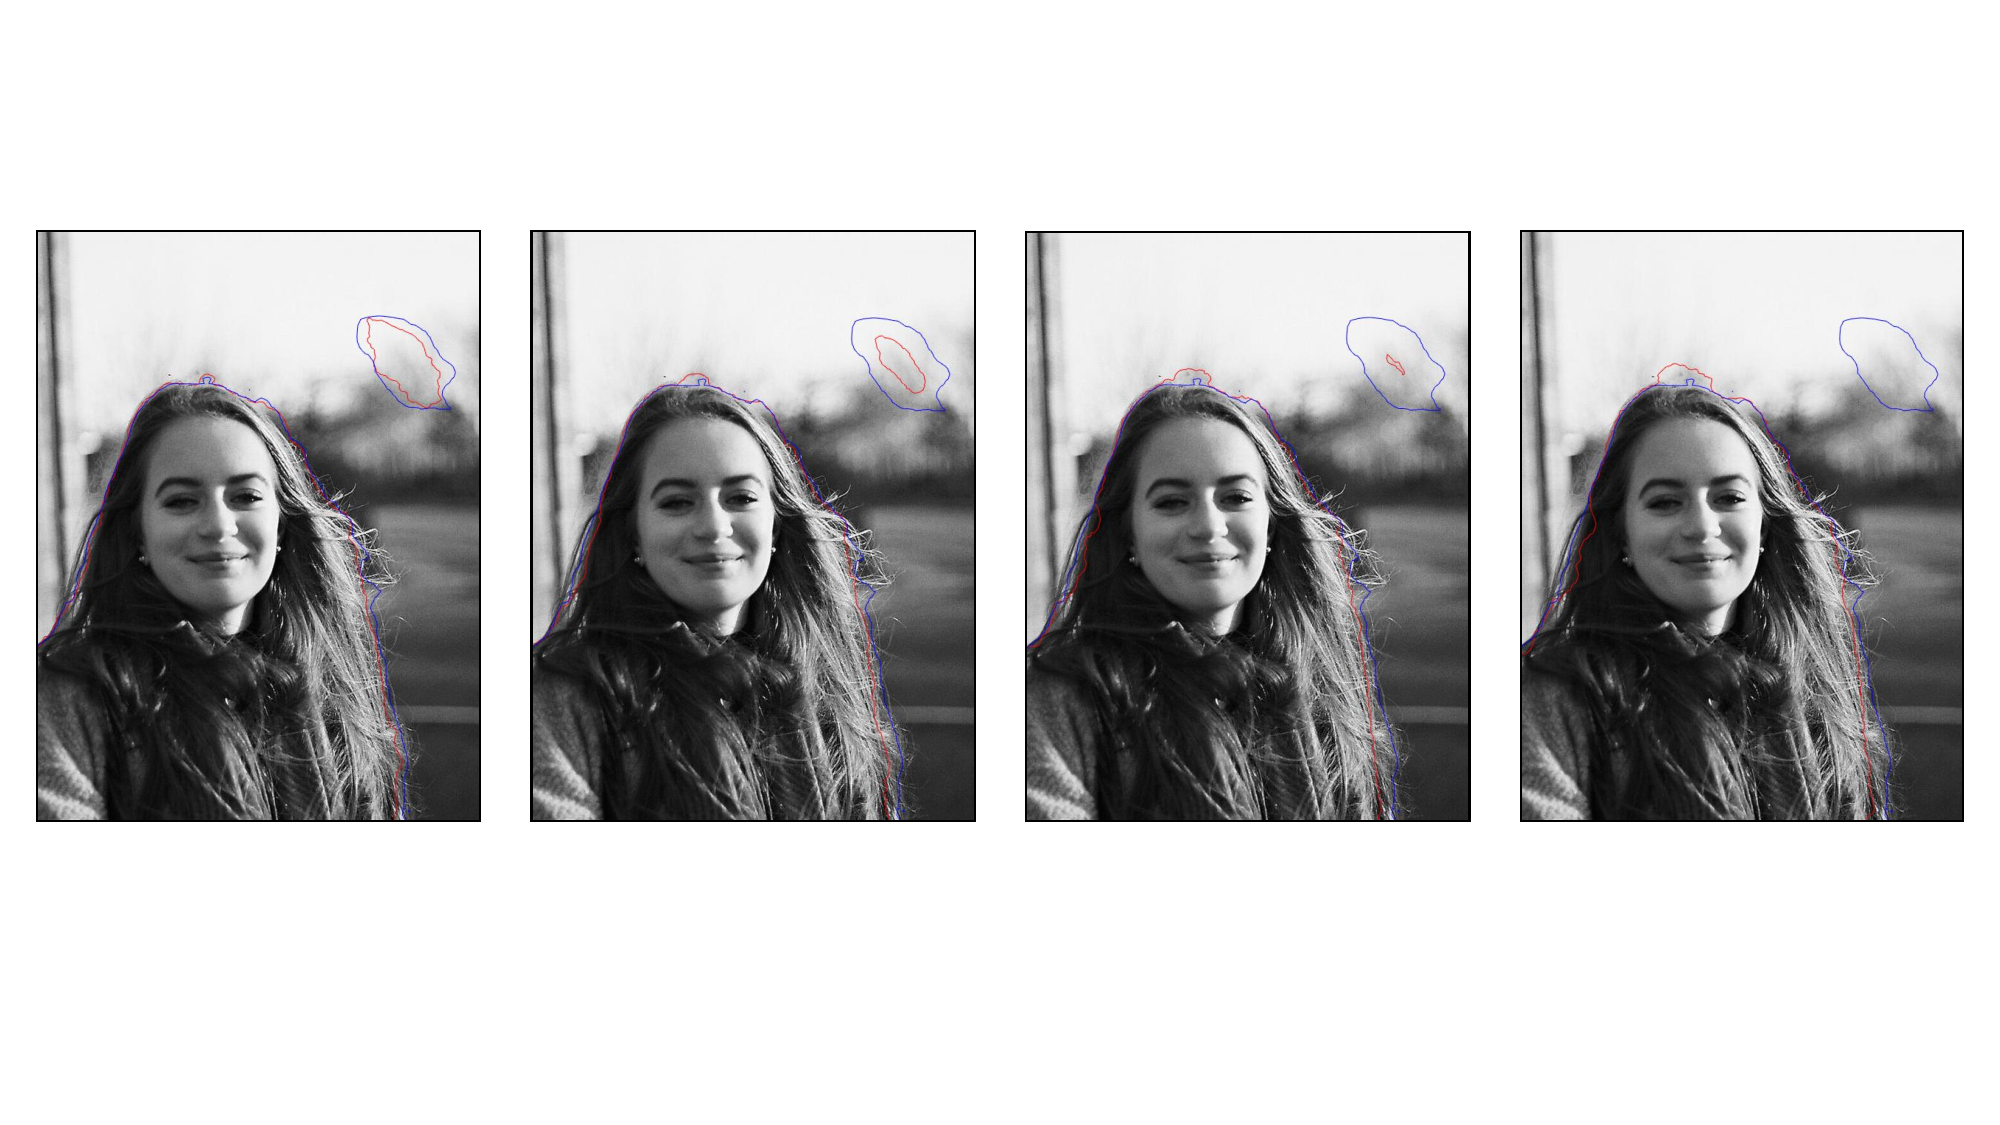
\includegraphics[width=9cm]{figs/Experiment1Result.eps}
    \caption{The contour evolution process of Experiment $1$.}
    \label{fig: The contour evolution process of Experiment 1}
\end{figure}
From the experiment result, we can see that the final segmentation result is more similar to the corrected prior shape.

\subsubsection{Experiment $2$}
There are some differences between experiment $1$ and experiment $2$. In here, $\mathcal{E}_{\text{img}}$ only uses the original image information, making it easier to capture the boundaries in the original picture.
\begin{equation*}
\begin{split}
    \mathcal{E}_{\text{img}} & = \\
    & \sum_{i=1}^2 \lambda_i\int \left( \int K_\sigma(\mathbf{x}-\mathbf{y}) \left| I(\mathbf{y}) - f_i(\mathbf{x}) \right|^2 M_i(\phi(\mathbf{y}))\mathrm{d}\mathbf{y} \right)\mathrm{d}\mathbf{x}
\end{split}
\end{equation*}
And $\mathcal{E}_{\text{shape}}$ uses the product of the probability map and the corrected prior shape $Q_i(\mathbf{x}) = P_i(\mathbf{x})\cdot Smooth(S_i(\mathbf{x}))$, $Smooth(S_i(\mathbf{x}))$ is the average smooth of the corrected prior shape. The result of product is shown in Fig. \ref{fig: The product of the probability map and the corrected prior shape}.
\begin{figure}[h]
    \centering
    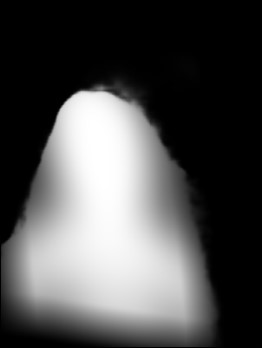
\includegraphics[width=3cm]{figs/Experiment2_plus.jpg}
    \caption{The product of the probability map and the corrected prior shape.}
    \label{fig: The product of the probability map and the corrected prior shape}
\end{figure}
Now, $\mathcal{E}_{\text{shape}}$ is redefined as follows
\begin{equation*}
    \mathcal{E}_{\text{shape}} = \sum_{i=1}^2 \pi_i \int Q_i(\mathbf{x}) M_i(\phi(\mathbf{x})) \mathrm{d}\mathbf{x}
\end{equation*}
Experiment $2$ is equivalent to using the intersection of the probability map and the corrected shape prior as the target shape regions, and then the boundary of target is located according to the information of the original image. The contour evolution process of Experiment $2$ is shown in Fig. \ref{fig: The contour evolution process of Experiment 2}.
\begin{figure}[h]
    \centering
    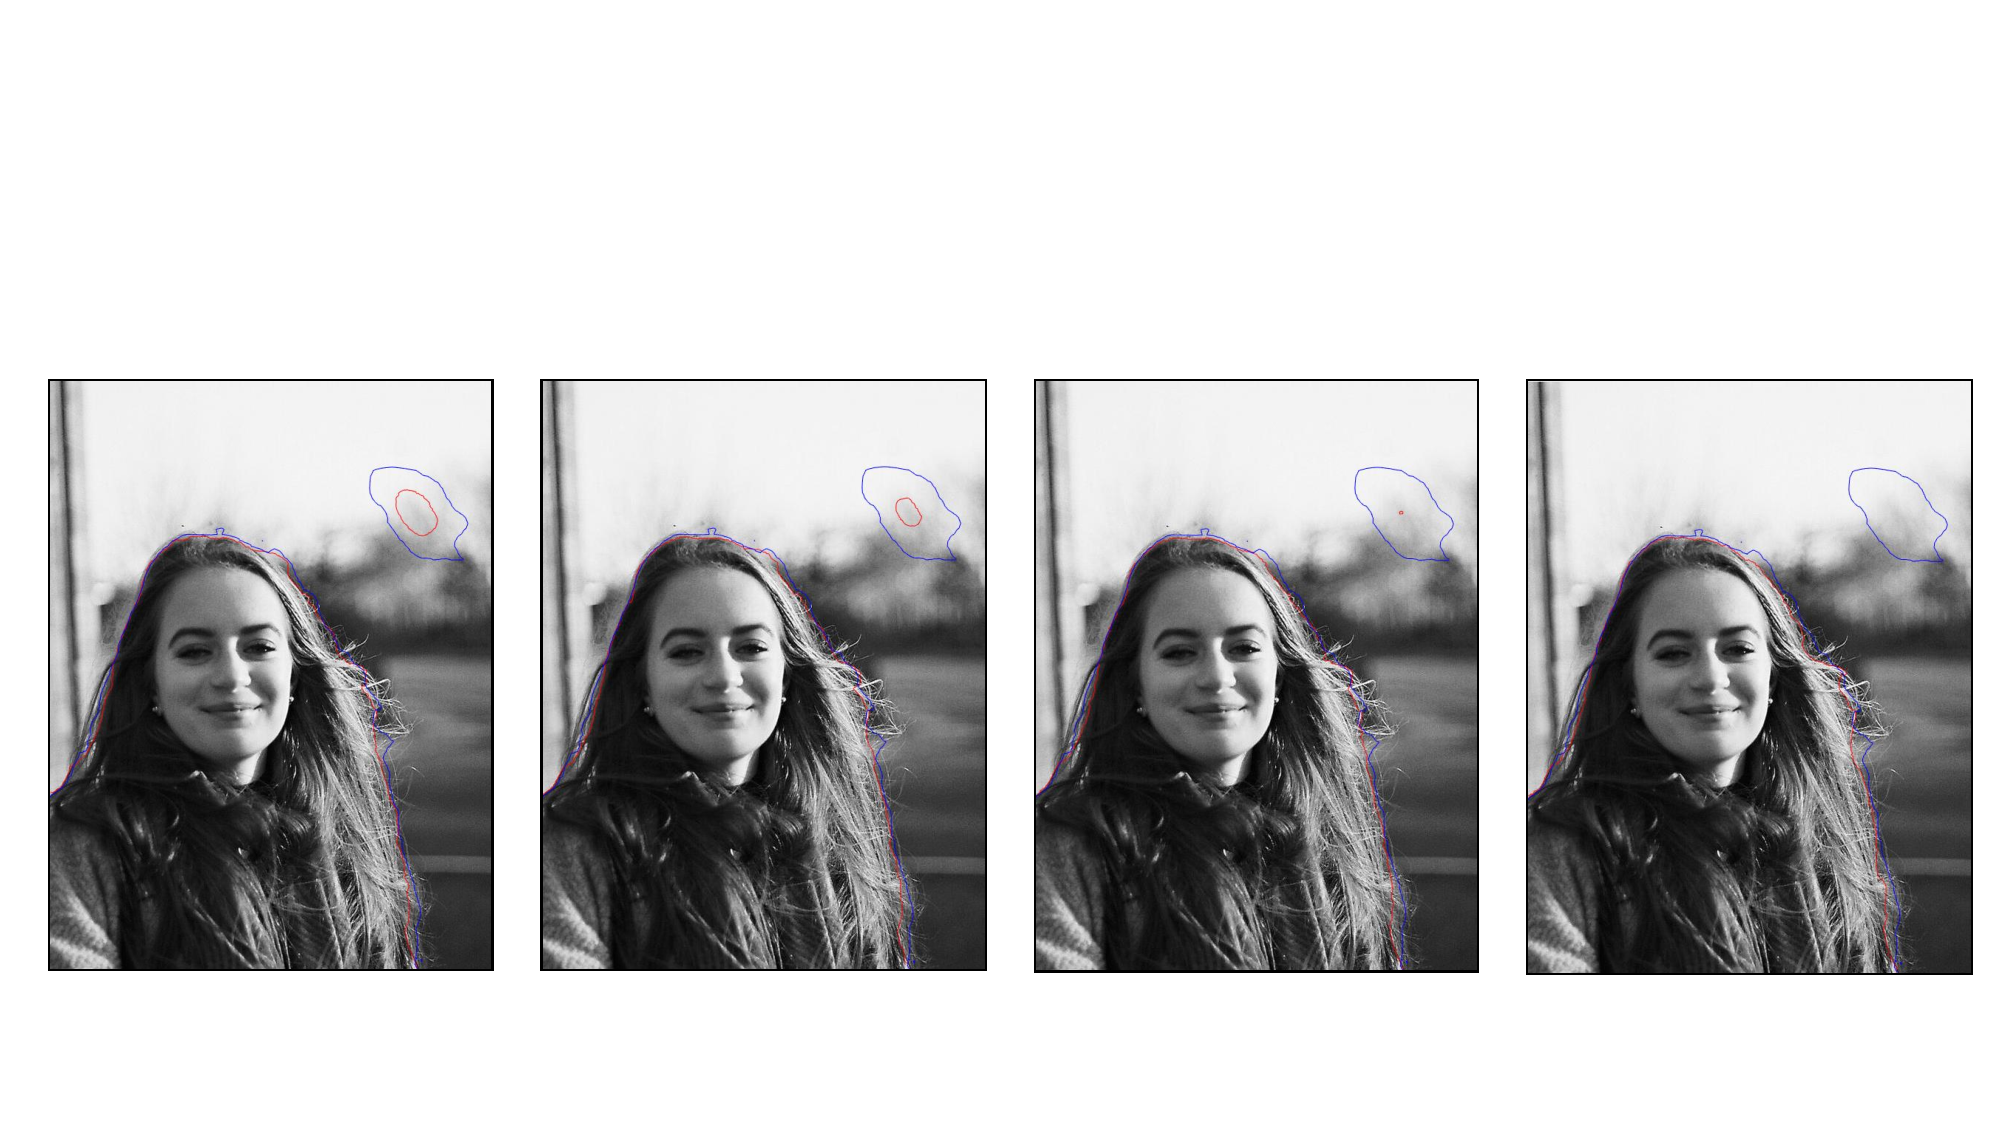
\includegraphics[width=9cm]{figs/Experiment2Result.eps}
    \caption{The contour evolution process of Experiment $2$.}
    \label{fig: The contour evolution process of Experiment 2}
\end{figure}
It can be seen that this method works better in this image, and it can more accurately locate the boundary of the target.
